\documentclass{ctexart}

\usepackage{amsmath}

\usepackage{amsthm}

\usepackage{amssymb}

\usepackage{bm}

\usepackage{graphicx}

\usepackage{listings}
\lstset{
basicstyle=\scriptsize
}

\usepackage{caption}

\begin{titlepage}

\title{微分方程数值解 \\ 第十三周作业}

\author{于慧倩 \\ 14300180118}

\date{2017年6月}
\end{titlepage}

\begin{document}

\maketitle

\newpage

\begin{enumerate}

\item P195 (4.2.16)

证明Richardson格式:
$$
\frac{u_i^{n+1}-u_i^{n-1}}{2 \tau} = a \Delta_h u_i^n+f_i^n
$$

的截断误差为$O(\tau^2+h^2)$

\begin{proof}

在$(t_n,x_i)$的截断误差为:

$$
R_i^n = \frac{u(t_{n+1},x_i)-u(t_{n-1},x_i}{2 \tau} - a \Delta_h u(t_n,x_i) -a\Delta_hu(t_n,x_i)-f(t_n,x_i)
$$

代入$f(t_n,x_i)$的表达式,有

\begin{eqnarray*}
R_t &=& \frac{u(t_{n+1},x_i)-u(t_{n-1},x_i}{2 \tau}-\frac{\partial u(t_n,x_i)}{\partial t} \\
&=& \frac{\tau^2}{6} \frac{\partial^3 u(t_n,x_i)}{\partial t^3} +O(\tau^4)
\end{eqnarray*}

\begin{eqnarray*}
R_x &=& -a\Delta_h u(t_n,x_i)+a\Delta u(t_n,x_i)\\
&=& -\frac{ah^2}{12}\frac{\partial^4 u(t_n,x_i)}{\partial x^4}+O(h^4)
\end{eqnarray*}

所以有

$$
R_i^n= \frac{\tau^2}{6} \frac{\partial^3 u(t_n,x_i)}{\partial t^3}  -\frac{ah^2}{12}\frac{\partial^4 u(t_n,x_i)}{\partial x^4}+O(h^4)+O(\tau^4)
$$


\end{proof}

\item P195 1

用$\theta$格式和Richardson格式求解抛物型方程,其中我们设真实解为$u(t,x)=\mbox{sin}(\pi x) e^{-\pi^2 t}$,观察差分格式收敛的情况。并当$t \rightarrow \infty$时,计算得到的解与两点边值问题的解是否一致?

取$X \in [0,1],T \in [0,1]$分别作出真解、$\theta=0,1,\frac{1}{2}$、以及Richardson格式的解如下图所示:

\centerline{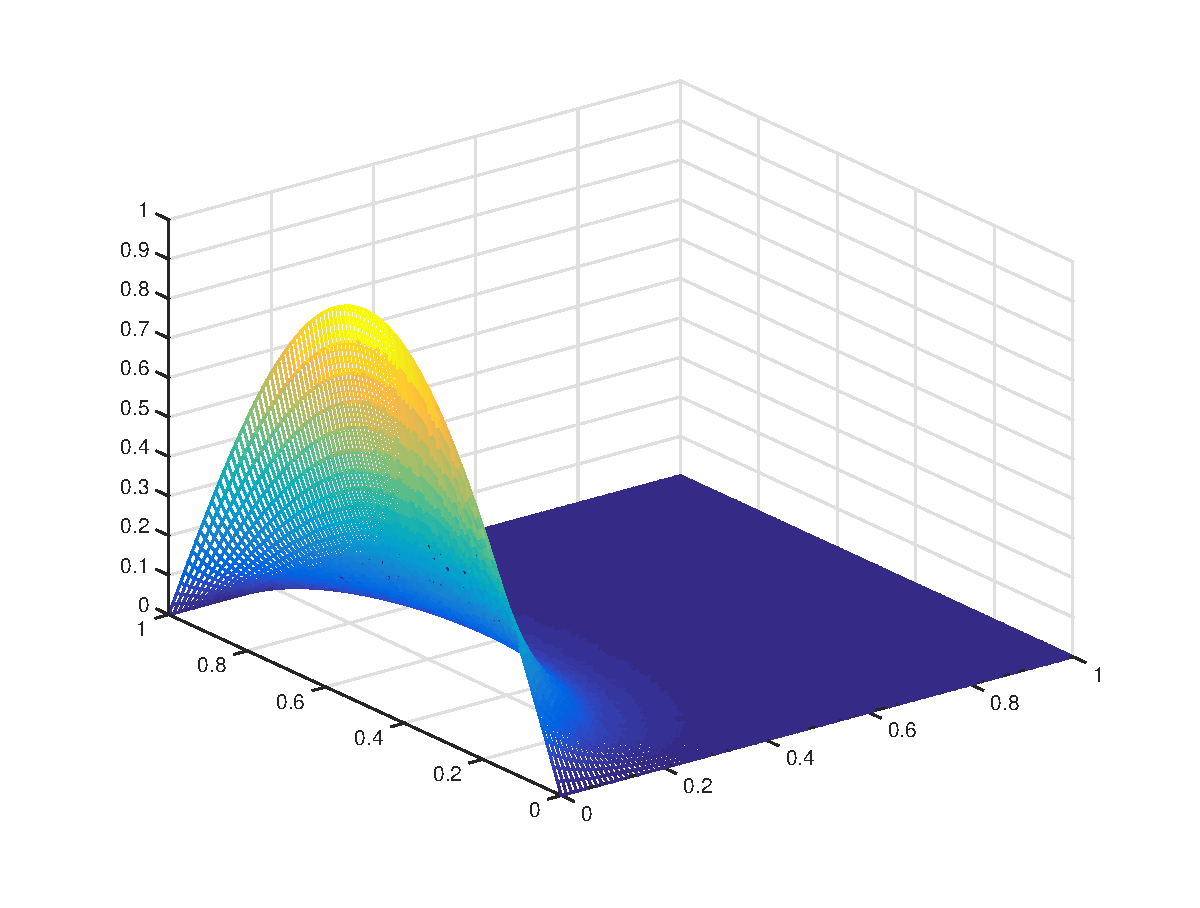
\includegraphics[width=5in]{H13_2_1.eps}}

\centerline{\includegraphics[width=5in]{H13_2_2.eps}}

\centerline{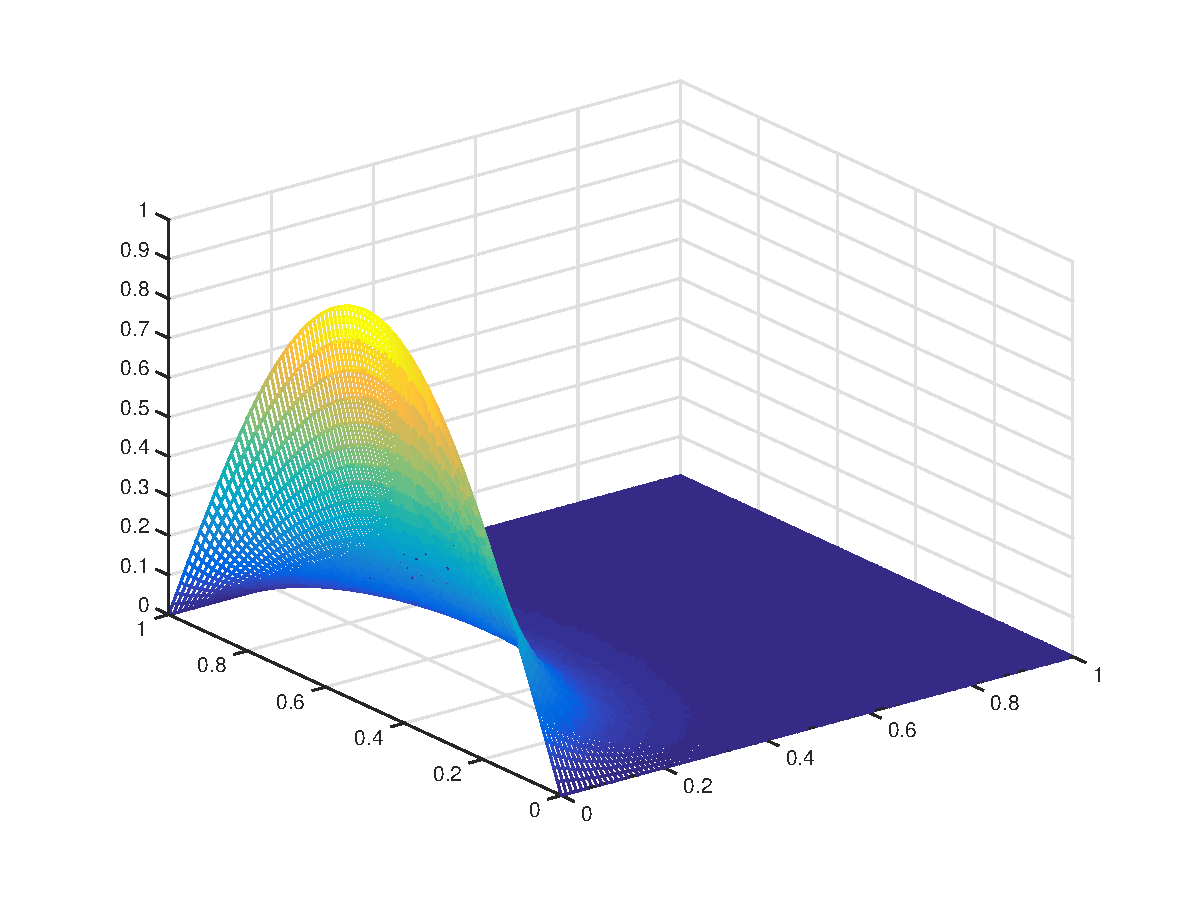
\includegraphics[width=5in]{H13_2_3.eps}}

\centerline{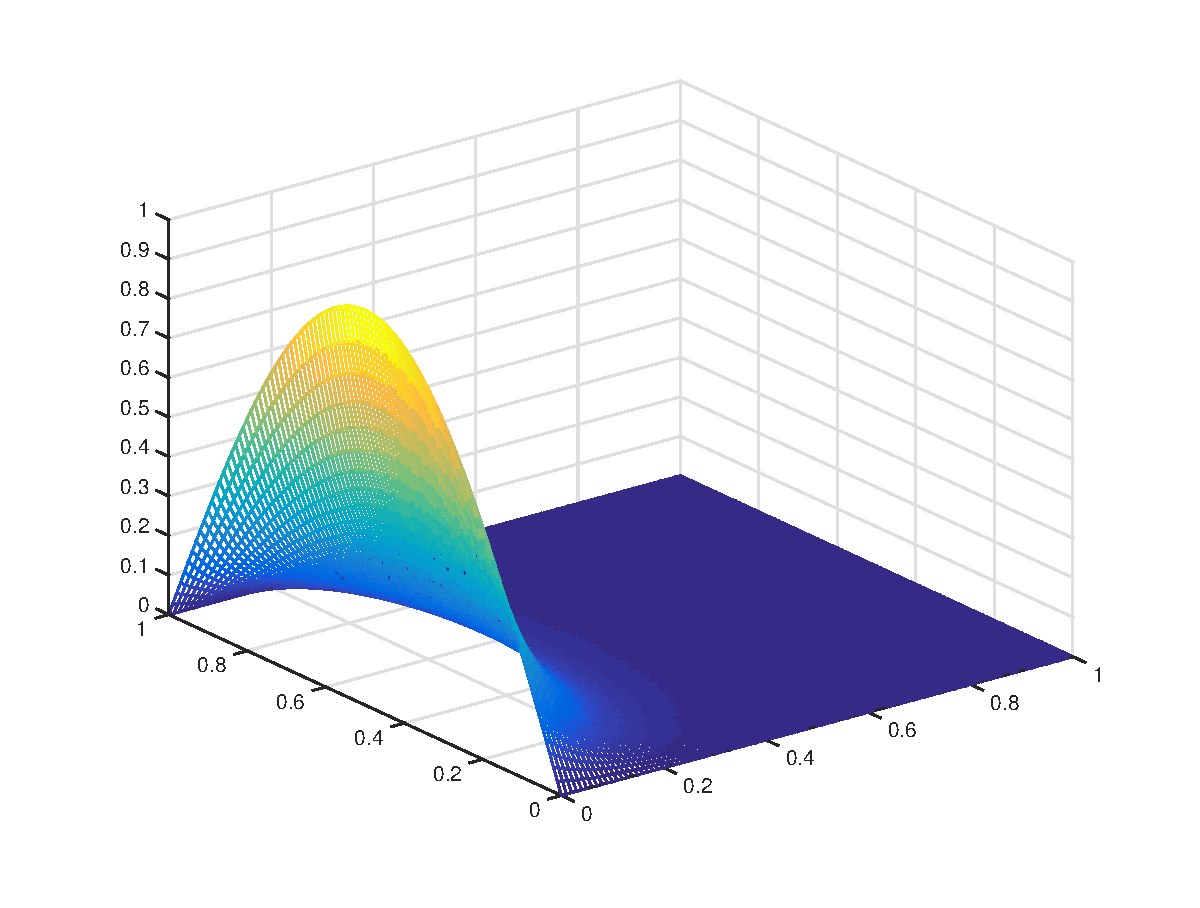
\includegraphics[width=5in]{H13_2_4.eps}}

\centerline{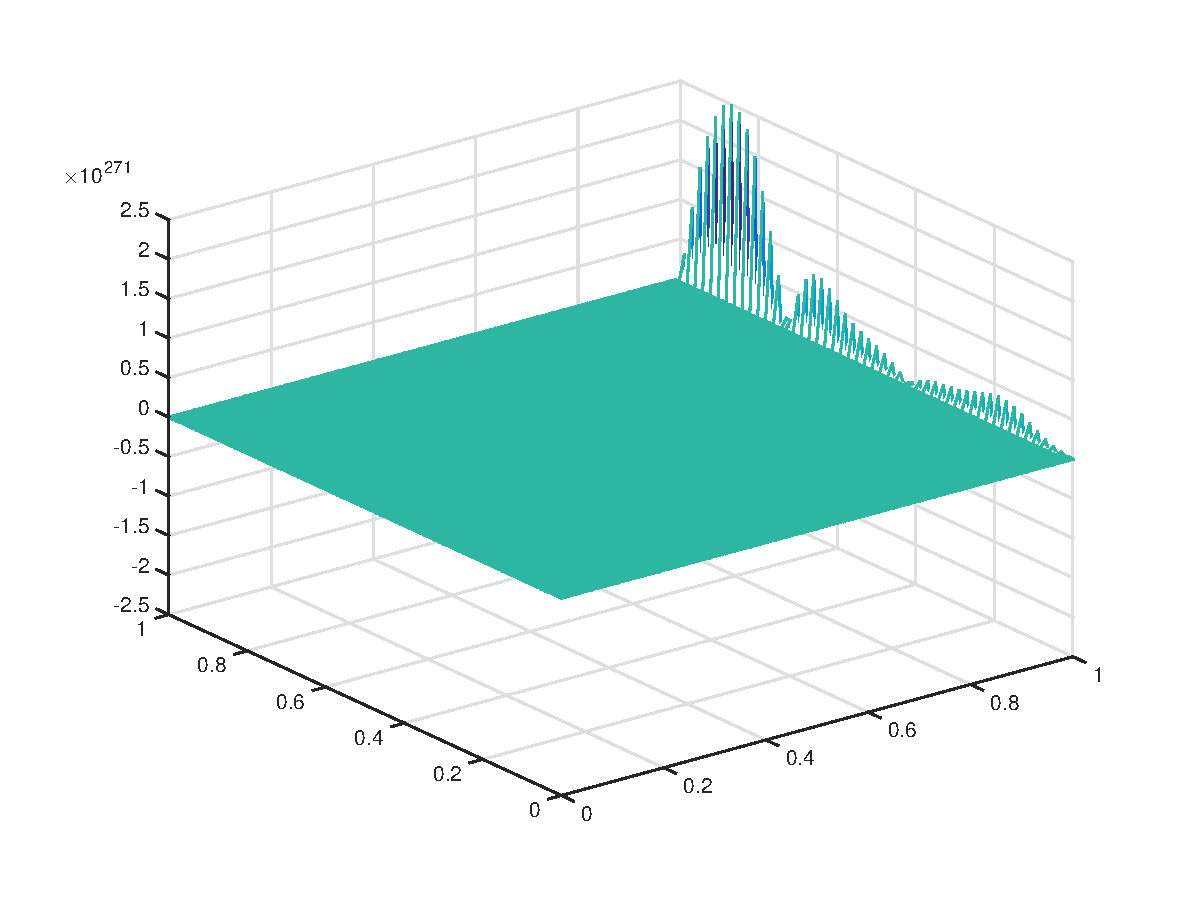
\includegraphics[width=5in]{H13_2_5.eps}}

并作出$\theta=0,1,\frac{1}{2}$以及Richardson格式误差图如下所示:

\centerline{\includegraphics[width=5in]{H13_2_0.eps}}

\centerline{\includegraphics[width=5in]{H13_2_11.eps}}

\centerline{\includegraphics[width=5in]{H13_2_55.eps}}

\centerline{\includegraphics[width=5in]{H13_2_66.eps}}

如图可以看到,$\theta=0$以及Richardson格式是不稳定的,当$t \rightarrow \infty$时,计算得到的解与两点边值问题的解不一致,而其他情况是收敛且与两点边值问题一致的。







\end{enumerate}
\end{document}